\section{实验结果与分析}

本章节将介绍本次实验的结果与分析,包括实验结果的展示,消融实验的结果,实验结果的分析等。

\subsection{实验结果}

图\ref{fig:result}展示了Tiny Image表征和Bag of Words表征的混淆矩阵:

% 并排两张子图,在pics目录中,tiny_image_confusion_matrix.png / bag_of_words_confusion_matrix.png
\begin{figure}[H]
    \centering
    \subfigure[Tiny Image表征的混淆矩阵]{
        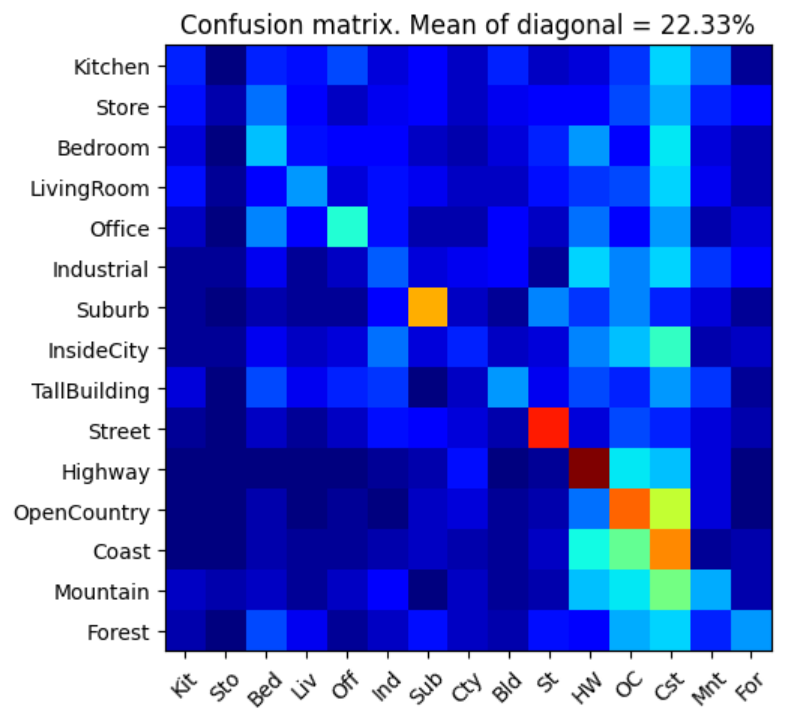
\includegraphics[width=0.45\textwidth]{pics/tiny_image_confusion_matrix.png}
    }
    \subfigure[Bag of Words表征的混淆矩阵]{
        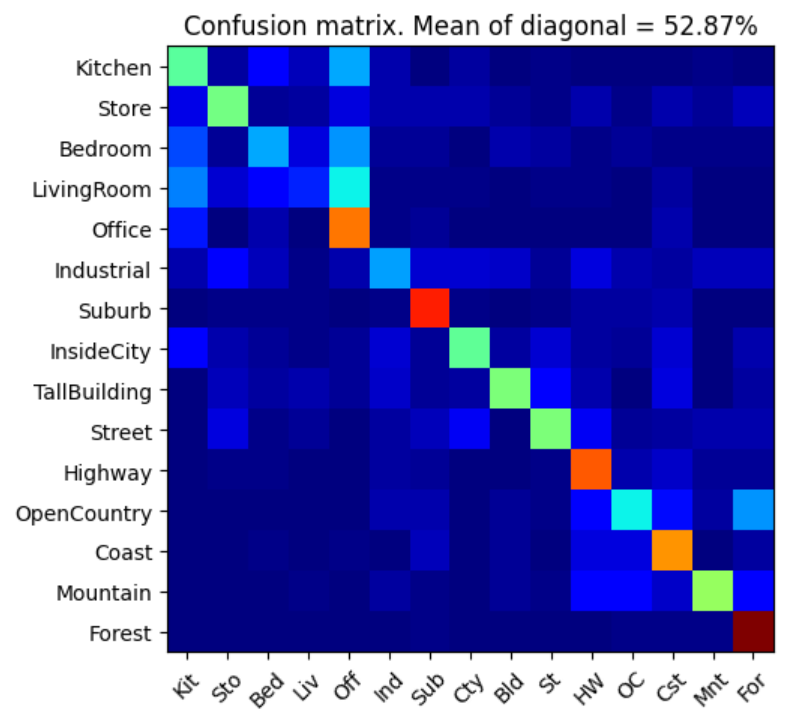
\includegraphics[width=0.45\textwidth]{pics/bag_of_words_confusion_matrix.png}
    }
    \caption{实验结果}
    \label{fig:result}
\end{figure}

从图中可以看出,基于Tiny Image表征KNN分类准确率为22.33\%,而基于Bag of Words表征KNN分类准确率为52.87\%,因此Bag of Words表征的效果明显优于Tiny Image表征。此外,从混淆矩阵中可以看出,Bag of Words混淆矩阵的对角线元素颜色更深,说明Bag of Words表征的分类效果更好。对角线元素的颜色越浅,说明该类别的分类难度越大,尤其是Bedroom、Living Room之间非常容易混淆,以及Industrial、OpenCountry也是非常难分的类别。

\subsection{消融实验}

为了分析Bag of Words表征的一些关键参数对分类准确率的影响,本章节展示消融实验,包括词典大小、K值、特征提取步长等参数的影响。图\ref{fig:ablation}展示了消融实验的结果:

% 并排3张子图,vocab_size_vs_accuracy.png / stride_vs_step_size_vs_accuracy.png / k_vs_accuracy.png
\begin{figure}[H]
    \centering
    \subfigure[词典大小对准确率的影响]{
        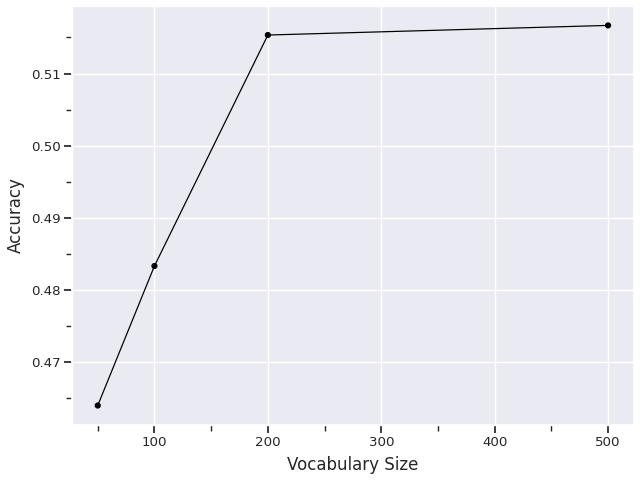
\includegraphics[width=0.45\textwidth]{pics/vocab_size_vs_accuracy.png}
    }
    \subfigure[K值对准确率的影响]{
        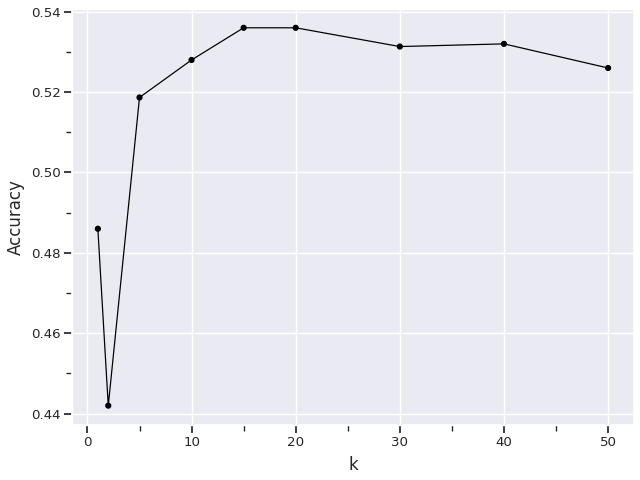
\includegraphics[width=0.45\textwidth]{pics/k_vs_accuracy.png}
    }
    \\
    \subfigure[步长对准确率的影响]{
        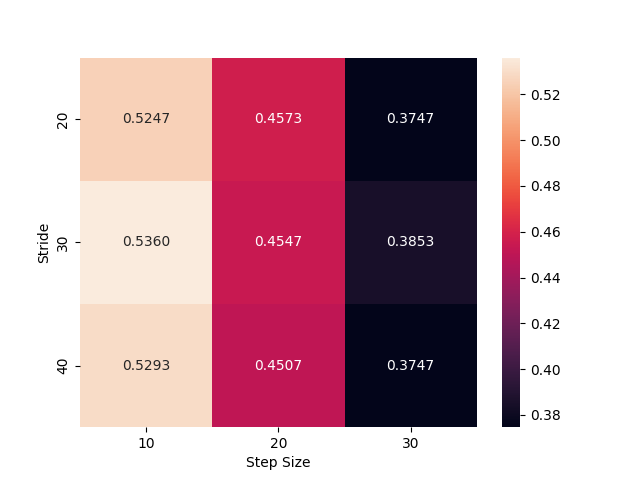
\includegraphics[width=0.5\textwidth]{pics/stride_vs_step_size_vs_accuracy.png}
    }
    \caption{消融实验}
    \label{fig:ablation}
\end{figure}

从子图(a)中可以看出,词典大小对分类准确率有较大的影响,随着词典大小的增加,分类准确率逐渐提高,但当词典大小达到500后,分类准确率逐渐饱和。因此,词典大小的选择需要在准确率和计算复杂度之间进行权衡。从子图(b)中可以看出,K值对分类准确率有较大的影响,K取15~20时效果最佳,小于15或大于20的K值性能都有所下降。

从子图(c)中可以看出,提取词典特征的步长大小对分类效果影响不大,而提取训练和测试图像特征的步长大小对分类效果影响较大,最终选择词典特征步长为30,图像特征步长为10的提取方案。虽然更小的步长可以提取更多的特征,但是计算复杂度和内存消耗也会显著增加,出于性能考虑,这里并没有选择更小的步长。

需要注意的是,消融实验中的最优结果与实验结果有所不同,这是因为KMeans等算法存在一定的随机性。

\subsection{实验分析}

本实验使用Tiny Image表征和Bag of Visual Words表征对图像进行分类,实验结果表明Bag of Visual Words表征的分类效果明显优于Tiny Image表征。

Tiny Image表征方法是一种简单的图像表征方法,将图像缩放至固定大小,然后展开为一个向量。虽然Tiny Image表征简单易实现,但是这种方法对图像特征的抽取能力非常有限。这是因为:

\begin{itemize}
    \item Tiny Image表征忽略了图像的空间信息,将图像展开为一个向量,丢失了图像的空间结构信息。
    \item Tiny Image表征对图像进行高度缩放,损失了大量的图像细节信息。
    \item Tiny Image表征对图像的光照、旋转、尺度变化等因素非常敏感,只要图像发生微小的变化,Tiny Image表征就会完全不同,因为它只是简单地将图像展开为一个向量。
\end{itemize}

相比之下,Bag of Visual Words表征方法克服了Tiny Image表征的这些缺点,它通过构建词典、提取图像特征、构建直方图等步骤,有效地提取了图像的局部特征,从而实现了更好的分类效果。

之所以Bag of Visual Words能有效表示图像,是因为它将图像视为由局部特征构成的集合,而不是简单地将图像展开为一个向量。现实场景中的图像通常是由各种各样的局部特征组成的,例如一辆车的图像中包含车轮、车窗、车身等局部特征,而不同类别的车通常具有不同的局部特征。受到文本检索中词典模型的启发,Bag of Visual Words将图像中的局部特征进行聚类,提取高度概括性的视觉词。之后就可以通过统计图像中的视觉词出现次数,构建直方图,实现图像的表征。

Bag of Visual Words表征方法的优点是:

\begin{itemize}
    \item Bag of Visual Words表征充分利用了图像的局部特征,将图像抽象为字典中的词频集合,对图像的空间信息、尺度信息、光照信息等具有较好的不变性。
    \item Bag of Visual Words表征具有较好的可解释性,可以通过查看图像的直方图,了解图像的局部特征分布情况。
    \item Bag of Visual Words表征具有较好的泛化能力,适用于不同场景、不同数据集的图像分类任务。
\end{itemize}

然而,Bag of Visual Words表征方法也存在一些缺点:

\begin{itemize}
    \item Bag of Visual Words表征需要事先构建视觉词典,这需要大量的计算和存储资源,且对词典的质量要求较高。
    \item Bag of Visual Words表征对特征提取算法要求较高,需要选择合适的特征提取算法。
    \item Bag of Visual Words表征只统计了图像中局部特征的出现次数,没有统计特征之间的空间关系。
\end{itemize}

如今,随着深度学习的发展,深度学习模型在图像分类、目标检测、图像分割等领域取得了巨大成功,传统的图像表征方法逐渐被深度学习模型所取代。然而,传统的图像表征方法仍然有很多值得探究的地方,给深度学习提供了很大启发。例如,深度学习模型中原型和记忆网络的设计,就和Bag of Words的思想非常相似,都是通过有限数量的“单词”概括特征。即便在高度发展的大模型中,也有将图像分割为patch,以及为patch或单词学习一个向量的Word Embedding思想。因此,传统的图像表征方法仍然是现在计算机视觉领域不可或缺的知识。

此外,传统的图像表征方法在可解释性上具有优势,可以通过查看直方图、词典等方式,了解图像分类的原理。而深度学习模型通常是一个黑盒模型,很难解释其分类原理。因此,传统的图像表征方法在一些对可解释性要求较高的场景中仍然具有一定的优势。